
% Lecture Template for ME3001-001-Tristan Hill - Spring 2017 - Fall 2017 - Fall 2020
% Mechanical Engineering Analysis with MATLAB
% Module 1 - Introduction 
% Topic 1 - What is Analysis ?

% Document settings

%\documentclass{beamer}                  % for presentation ?
\documentclass[handout]{beamer}  % for handout ?
\usepackage{/home/thill/Documents/lectures/analysis_lectures/analysis_lectures}

\newcommand{\MNUM}{1\hspace{2mm}} % Module number
\newcommand{\TNUM}{1\hspace{2mm}} % Topic number 
\newcommand{\moduletitle}{Introduction and MATLAB Review} % Titles and Stuff
\newcommand{\topictitle}{Introduction to Analysis} 

\newcommand{\sectiontitleI}{What is this class about?} % More Titles and Stuff
\newcommand{\sectiontitleII}{How does it apply to mechanical engineering?}
\newcommand{\sectiontitleIII}{What areas of engineering will we cover?}
\newcommand{\sectiontitleIV}{Remember those math classes? }
\newcommand{\sectiontitleV}{Major Topics Covered }

\newcommand{\btVFill}{\vskip0pt plus 1filll}

% custom box
\newsavebox{\mybox}

\author{ME3001 - Mechanical Engineering Analysis}  
\title{Lecture Module - \moduletitle}
\date{Mechanical Engineering\vspc Tennessee Technological University}

\begin{document}
	
	\lstset{language=MATLAB,basicstyle=\ttfamily\small,showstringspaces=false}
	
	\frame{\titlepage \center\begin{framed}\Large \textbf{Topic \TNUM - \topictitle}\end{framed} \vspace{5mm}}
	
	% Section 0: Outline
	\frame{
		\large \textbf{Topic \TNUM - \topictitle} \vspace{3mm}\\
		
		\begin{itemize}
			
			\item \sectiontitleI    \vspc % Section I
			\item \sectiontitleII 	\vspc % Section II
			\item \sectiontitleIII 	\vspc %Section III
			\item \sectiontitleIV 	\vspc %Section IV
			
		\end{itemize}
		
	}
	

\section{\sectiontitleI}

\frame{
  \frametitle{\sectiontitleI}
  			
  			
    \begin{itemize}
		
		\item Analysis \vspace{15mm}
		
		\item Design

	\end{itemize}  

}

\frame{
	\frametitle{\sectiontitleI}
	
	Define {\it Analysis}: \\	
	- detailed examination of the elements or structure of something, typically as a basis for discussion or interpretation. {\tiny -\href{https://www.merriam-webster.com/dictionary/analysis}{Merriam-Webster}} \vspace{5mm} \\ 

	Define {\it Design}: \\
	- A design is a plan or specification for the construction of an object or system or for the implementation of an activity or process, or the result of that plan or specification in the form of a prototype, product or process. The verb to design expresses the process of developing a design. {\tiny -\href{https://en.wikipedia.org/wiki/Design}{Wikipedia}}\\
	
}

\section{\sectiontitleII}

\frame{
  \frametitle{\sectiontitleII}
  
  \textbf{This is not just another math class!}\\


	\begin{itemize}
			\item we will study mathematical modeling of engineering systems and the theoretical and numerical solutions to non-linear equations, systems of linear equations, and ordinary and partial differential equations \\
			
			\item mathematical methods for solving mechanical engineering problems with modern computing tools\\
    
		
		\item we can solve the \large{BIG} problems!

	\end{itemize}  

}
\section{\sectiontitleIII}

\frame{
  \frametitle{\sectiontitleIII}
	
	\begin{itemize}
	
		\item Statics and Mechanics\\
		\item Rigid Body Dynamics\\
		\item Fluid Dynamics\\
		\item Thermodynamics and Heat Transfer\\
		\item Vibrations\\
	
	\end{itemize}  

}
\section{\sectiontitleIV}

\frame{
  \frametitle{\sectiontitleIV}
  
	We will be doing some {\it applied mathematics} in this class!
	\begin{multicols}{2}
	\begin{itemize}
	
		\item Algebra and Arithmetic\\
		\item Matrix\slash Linear Algebra \\
		\item Calculus \\
		\item Ordinary and Partial \\Differential Equations \\
		\item The Fourier Series \\
		
	
	\end{itemize}
	\end{multicols} 

}

\frame{
  \frametitle{\sectiontitleIV}
		This class is different than a traditional mathematics class.\\ 
				\begin{itemize}
					\item By nature engineering problems are hard to solve on paper.\\
					
					\item So, will be using calculators but we will also be using...\\
									
					\item \hspace{1mm} \vspace{10mm}\\
									
				\end{itemize}
				
		 Modern Computing Tools\\ 		
		
				\begin{itemize}
					\item  \hspace{1mm} \vspace{5mm}\\
					
					\item  \hspace{1mm} \vspace{5mm}\\
					
					\item  \hspace{1mm} \vspace{5mm}\\
									
				\end{itemize}
		
	}



\section{\sectiontitleV}

\frame{
  \frametitle{\sectiontitleV}	
   \begin{enumerate}
					\item Computer Programming for Scientific Computation \hspace{1mm} \vspace{3mm}\\
					
					\item Solutions to Non-Linear Equations \hspace{1mm} \vspace{3mm}\\
					
					\item Solving Systems of Linear Equations \hspace{1mm} \vspace{3mm}\\
					
					\item Numerical Integration and Curve Fitting \hspace{1mm} \vspace{3mm}\\
					
					\item Ordinary Differential Equations \hspace{1mm} \vspace{3mm}\\
					
					\item Partial Differential Equations
									
	\end{enumerate}
  
  }
  \frame{
  \frametitle{\sectiontitleV}	
  1) Computer Programming for Scientific Computation
   \begin{itemize}
					\item  \hspace{1mm} \vspace{3mm}\\
					
					\item  \hspace{1mm} \vspace{3mm}\\
					
					\item \hspace{1mm} \vspace{3mm}\\
					

									
	\end{itemize}
  
  }
  \frame{
  \frametitle{\sectiontitleV}	
   2) Solutions to Non-Linear Equations \vspace{5mm}\\
				\begin{itemize}
					\item Rigid Body Dynamics \\
					
					\item Optimization and Design \\
					
				\end{itemize}
  
  }
    \frame{
  \frametitle{\sectiontitleV}	
   3) Solving Systems of Linear Equations \vspace{5mm}\\
			\begin{multicols}{2}
				\begin{itemize}
					\item Statics and Structural  \\
					
					\item Equilibrium Equations\\
					
					\item The Eigenvalue Problem\\
					
					\item Mechanisms and Machines\\
					
				\end{itemize}
				\end{multicols}
  }
    \frame{
  \frametitle{\sectiontitleV}	
   4) Numerical Integration and Curve Fitting \vspace{5mm}\\
				\begin{itemize}
					\item 
					
					\item 
					
				\end{itemize}
  
  }
     \frame{
  \frametitle{\sectiontitleV}	
   5) Ordinary Differential Equations \vspace{5mm}\\
	\begin{itemize}
					\item What is a Differential Equations? What about a system of them?\vspace{5mm} \\
					\item What does it mean to solve a differential equation? \vspace{5mm} \\
					\item A very simple example:
					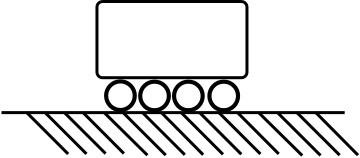
\includegraphics[scale=.2]{lecture1_fig3.png}\vspace{5mm}\\
					{ODE:}\vspace{5mm}\\
					{Solution:}\\
			\end{itemize}
  }
   \frame{
  \frametitle{\sectiontitleV}	
   6) Partial Differential Equations \vspace{5mm}\\
			\begin{itemize}
					\item What is different about a Partial Differential Equation? \vspace{5mm} \\
					
					\item What is different about the solution to a PDE?  \vspace{5mm}  \\
					
					\item What does this allow us to do? \\
					
			\end{itemize}
  
  }
\end{document}
%
%	 Mathematical Modeling of Engineering Problems Involving: \\
%		\begin{enumerate}
%			\item Solutions to Non-Linear Equations \vspace{5mm}\\
%				\begin{itemize}
%					\item Rigid Body Dynamics \\
%					
%					\item Optimization and Design \\
%					
%				\end{itemize}
%			
%			\item Solving Systems Linear Equations \vspace{5mm}\\
%				\begin{multicols}{2}
%				\begin{itemize}
%					\item Statics and Structural  \\
%					
%					\item Equilibrium Equations\\
%					
%					\item The Eigenvalue Problem\\
%					
%					\item Mechanisms and Machines\\
%					
%				\end{itemize}
%				\end{multicols}
%			\item Ordinary Differential Equations \vspace{5mm}\\
%				\begin{multicols}{2}
%				\begin{itemize}
%					\item Rigid Body Dynamics\\
%					\item Thermodynamics and Heat Transfer\\
%					\item Electronics and Circuits\\
%				\end{itemize}
%				\end{multicols}
%			\item Partial Differential Equations \vspace{5mm}\\
%				\begin{itemize}
%					\item Fluid Dynamics\\
%					\item Thermodynamics and Heat Transfer\\
%				\end{itemize}
%		\end{enumerate}
%	\end{itemize}
%	\LARGE
%	\begin{enumerate}	
%		
%		\item \textbf{  Solutions to Non-Linear Equations}\\
%			\begin{itemize}
%					\item What is a non-linear equation? \vspace{20mm} \\
%					\item What does it mean to solve a non-linear equation? \vspace{20mm} \\
%					\item Standard form of this problem:\\
%					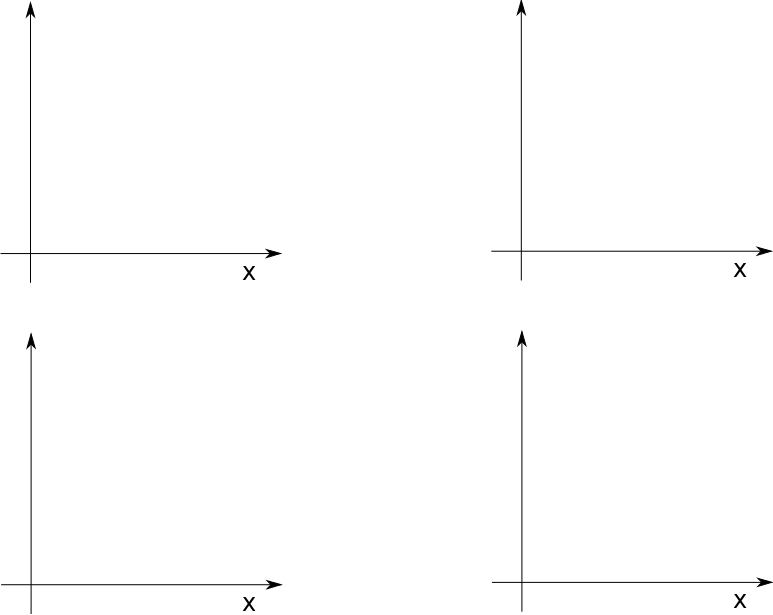
\includegraphics[scale=.5]{lecture1_fig1.png}
%			\end{itemize}
%\newpage			
%			\item \textbf{  Solving Systems Linear Equations}\\
%			\begin{itemize}
%					\item What is a system of linear equations?\vspace{20mm} \\
%					\item What does it mean to solve a  system of linear equations? \vspace{20mm} \\
%					\item A very simple example:\\
%					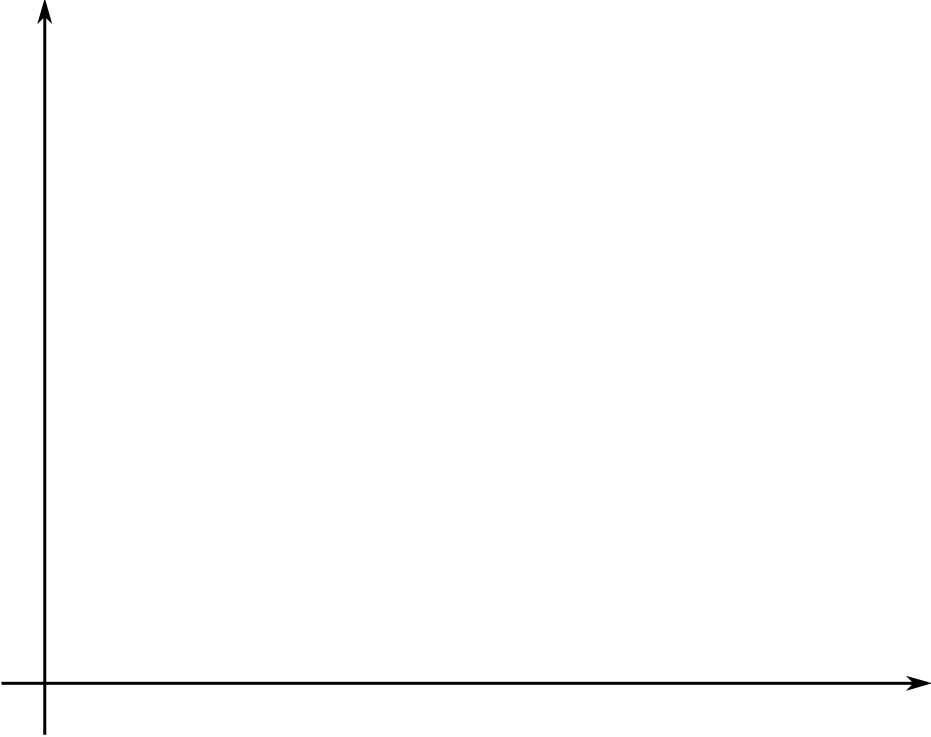
\includegraphics[scale=.45]{lecture1_fig2.png}
%			\end{itemize}
%			
%			\item \textbf{  Ordinary Differential Equations}\\
%			\begin{itemize}
%					\item What is a Differential Equations? What about a system of them?\vspace{20mm} \\
%					\item What does it mean to solve a differential equation? \vspace{20mm} \\
%					\item A very simple example:\\
%					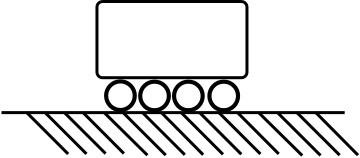
\includegraphics[scale=.6]{lecture1_fig3.png}\\
%					\Large {ODE:}\vspace{30mm}\\
%					\Large {Solution:}\\
%			\end{itemize}
%\newpage			
%			\item \textbf{  Partial Differential Equations}\\ 
%			\begin{itemize}
%					\item What is different about a Partial Differential Equation? \vspace{20mm} \\
%					
%					\item What is different about the solution to a PDE?  \vspace{20mm}  \\
%					
%					\item What does this allow us to do? \\
%					
%			\end{itemize}
%	\end{enumerate}
%		
%
%}
%
%	
%
%
%
%
%
